\documentclass[10pt,a4paper]{article}
\usepackage[UTF8,fontset = windows]{ctex}
\setCJKmainfont[BoldFont=黑体,ItalicFont=楷体]{华文中宋}
\usepackage{amssymb,amsmath,amsfonts,amsthm,mathrsfs,dsfont,graphicx}
\usepackage{ifthen,indentfirst,enumerate,color,titletoc}
\usepackage{tikz}
\usepackage{multicol}
\usepackage{makecell}
\usepackage{longtable}
\usepackage{diagbox}
\usetikzlibrary{arrows,calc,intersections,patterns,decorations.pathreplacing,3d,angles,quotes,positioning,shapes.geometric}
\usepackage[bf,small,indentafter,pagestyles]{titlesec}
\usepackage[top=1in, bottom=1in,left=0.8in,right=0.8in]{geometry}
\renewcommand{\baselinestretch}{1.65}
\newtheorem{defi}{定义~}
\newtheorem{eg}{例~}
\newtheorem{ex}{~}
\newtheorem{rem}{注~}
\newtheorem{thm}{定理~}
\newtheorem{coro}{推论~}
\newtheorem{axiom}{公理~}
\newtheorem{prop}{性质~}
\newcommand{\blank}[1]{\underline{\hbox to #1pt{}}}
\newcommand{\bracket}[1]{(\hbox to #1pt{})}
\newcommand{\onech}[4]{\par\begin{tabular}{p{.9\textwidth}}
A.~#1\\
B.~#2\\
C.~#3\\
D.~#4
\end{tabular}}
\newcommand{\twoch}[4]{\par\begin{tabular}{p{.46\textwidth}p{.46\textwidth}}
A.~#1& B.~#2\\
C.~#3& D.~#4
\end{tabular}}
\newcommand{\vartwoch}[4]{\par\begin{tabular}{p{.46\textwidth}p{.46\textwidth}}
(1)~#1& (2)~#2\\
(3)~#3& (4)~#4
\end{tabular}}
\newcommand{\fourch}[4]{\par\begin{tabular}{p{.23\textwidth}p{.23\textwidth}p{.23\textwidth}p{.23\textwidth}}
A.~#1 &B.~#2& C.~#3& D.~#4
\end{tabular}}
\newcommand{\varfourch}[4]{\par\begin{tabular}{p{.23\textwidth}p{.23\textwidth}p{.23\textwidth}p{.23\textwidth}}
(1)~#1 &(2)~#2& (3)~#3& (4)~#4
\end{tabular}}
\begin{document}

\begin{enumerate}[1.]
%gk10/23
\item 不等式$\dfrac{2-x}{x+4}>0$的解集是\blank{50}.
\item 若复数$z=1-2\mathrm{i}$($\mathrm{i}$为虚数单位), 则$z\cdot \overline z+z=$\blank{50}.
\item 动点$P$到点$F(2,0)$的距离与它到直线$x+2=0$的距离相等, 则$P$的轨迹方程为\blank{50}.
\item 行列式$\begin{vmatrix} \cos \dfrac{\pi }3 & \sin \dfrac{\pi }6 \\ \sin \dfrac{\pi }3 & \cos \dfrac{\pi }6 \end{vmatrix}$的值是\blank{50}.
\item 圆$C:x^2+y^2-2x-4y+4=0$的圆心到直线l:$3x+4y+4=0$的距离$d=$\blank{50}.
\item 随机变量$\xi$的概率分布率由下表给出: 
\begin{center}
\begin{tabular}{|c|c|c|c|c|}
\hline
$x$ & $7$ & $8$ & $9$ & $10$ \\ \hline
$P(\xi=x)$ & $0.3$ & $0.35$ & $0.2$ & $0.15$ \\ \hline
\end{tabular}
\end{center}
则随机变量$\xi$的均值是\blank{50}.
\item $2010$年上海世博会园区每天$9:00$开园, $20:00$停止入园. 在下面的框图中, $S$表示上海世博会官方网站在每个整点报道的入园总人数, $a$表示整点报道前$1$个小时内入园人数, 则空白的执行框内应填入\blank{50}.
\begin{center}
\begin{tikzpicture}[>=latex, node distance = 3ex]
\node [draw, rounded corners] (start) {开始};
\node [draw, below=of start]  (step1)  {$T\leftarrow 9$, $S\leftarrow 0$};
\node [draw, trapezium, trapezium right angle = 120, below=of step1]  (step2)  {输出$T,S$};
\node [draw, diamond, aspect = 3, below= of step2] (step3) {$T\le 19$};
\node [draw, below= of step3] (step4) {$T\leftarrow T+1$};
\node [draw,  trapezium, trapezium right angle = 120, below = of step4] (step5) {输入$a$};
\node [draw, below = of step5] (step6) {\phantom{$S\leftarrow S+a$}};
\node [right = of step3] (anchor2) {};
\node [below = of step6] (anchor3) {};
\node [draw, below = of anchor3] (end) {结束};
\node [left = of step3] (anchor1) {};
\draw[->] (start)  -- (step1);
\draw[->] (step1)  -- (step2);
\draw[->] (step2)  -- (step3);
\draw[->] (step3)  -- node[right] {是}(step4) ;
\draw[->] (step4)  -- (step5);
\draw[->] (step5)  -- (step6);
\draw[->] (step6) -- (anchor1|-step6) -- (anchor1|-step2) -- (step2);
\draw[->] (step3) --node[above] {否} (anchor2|-anchor2) -- (anchor2|-anchor3) -- (anchor3|-anchor3) -- (end);
\end{tikzpicture}
\end{center}
\item 对任意不等于$1$的正数$a$, 函数$f(x)=\log_a(x+3)$的反函数的图像都经过点$P$, 则点$P$的坐标是\blank{50}.
\item 从一副混合后的扑克牌($52$张)中随机抽取$1$张, 事件$A$为``抽得红桃K'', 事件$B$为``抽得为黑桃'', 则概率$P(A\cup B)=$\blank{50}.(结果用最简分数表示)
\item 在$n$行$n$列矩阵$\begin{pmatrix}
1 & 2 & 3 & \cdots &  n-2 & n-1 & n  \\ 2 & 3 & 4 & \cdots &  n-1 & n & 1  \\ 3 & 4 & 5 & \cdots &  n & 1 & 2  \\ \cdots &  \cdots &  \cdots &  \cdots  & \cdots &  \cdots &  \cdots   \\ n & 1 & 2 & \cdots &  n-3 & n-2 & n-1  \end{pmatrix}$中, 记位于第$i$行第$j$列的数为$a_{ij}$($i,j=1,2\cdots ,n$). 当$n=9$时, $a_{11}+a_{22}+a_{33}+\cdots +a_{99}=$\blank{50}.
\item 将直线$l_1:nx+y-n=0$、$l_2:x+ny-n=0$($n\in \mathbf{N}^*$, $n\ge 2$)$x$轴、$y$轴围成的封闭图形的面积记为$S_n$, 则$\displaystyle\lim_{n\to\infty} S_n=$\blank{50}.
\item 如图所示, 在边长为$4$的正方形纸片$ABCD$中, $AC$与$BD$相交于$O$, 剪去$\triangle AOB$, 将剩余部分沿$OC$、$OD$折叠, 使$OA$、$OB$重合, 则以$A(B)$、$C$、$D$、$O$为顶点的四面体的体积为\blank{50}.
\begin{center}
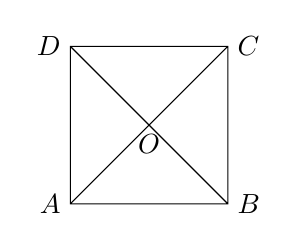
\begin{tikzpicture}[>=latex]
\draw (0,0) -- (2,2) (0,2) -- (2,0) (0,0) rectangle (2,2);
\draw (0,0) node [left] {$A$} coordinate (A);
\draw (2,0) node [right] {$B$} coordinate (B);
\draw (2,2) node [right] {$C$} coordinate (C);
\draw (0,2) node [left] {$D$} coordinate (D);
\draw (1,1) node [below] {$O$} coordinate (O);
\end{tikzpicture}
\end{center}
\item 如图所示, 直线$x=2$与双曲线$\Gamma :\dfrac{x^2}4-y^2=1$的渐近线交于$E_1$, $E_2$两点, 记$\overrightarrow{OE_1}=\overrightarrow{e_1}$, $\overrightarrow{OE_2}=\overrightarrow{e_2}$, 任取双曲线$\Gamma$上的点$P$, 若$\overrightarrow{OP}=a\overrightarrow{e_1}+b\overrightarrow{e_2}$($a,b\in \mathbf{R}$), 则$a$、$b$满足的一个等式是\blank{50}.
\begin{center}
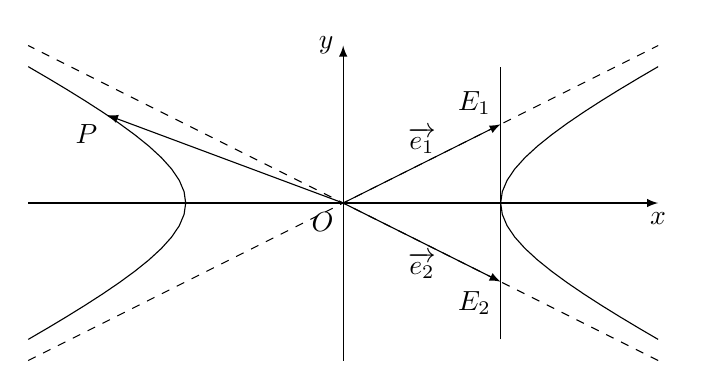
\begin{tikzpicture}[>=latex]
\draw [->] (-4,0) -- (4,0) node [below] {$x$};
\draw [->] (0,-2) -- (0,2) node [left] {$y$};
\draw (0,0) node [below left] {$O$};
\draw [dashed] (-4,-2) -- (4,2) (4,-2) -- (-4,2);
\draw [domain = {-sqrt(3)}:{sqrt(3)}] plot ({2*sqrt(1+pow(\x,2))},\x);
\draw [domain = {-sqrt(3)}:{sqrt(3)}] plot ({-2*sqrt(1+pow(\x,2))},\x);
\draw (2,{-sqrt(3)}) -- (2,{sqrt(3)});
\draw (2,1) node [above left] {$E_1$} coordinate (E1);
\draw (2,-1) node [below left] {$E_2$} coordinate (E2); 
\draw [->] (0,0) -- node [above] {$\overrightarrow{e_1}$} coordinate (e1) (E1);
\draw [->] (0,0) -- node [below] {$\overrightarrow{e_2}$} coordinate (e1) (E2);
\draw (-3,{sqrt(5/4)}) node [below left] {$P$} coordinate (P);
\draw [->] (0,0) -- (P);
\end{tikzpicture}
\end{center}
\item 在集合$U=\{a,b,c,d\}$的子集中选出$2$个不同的子集, 需同时满足以下两个条件: \textcircled{1} $a$、$b$都要选出; \textcircled{2} 对选出的任意两个子集$A$和$B$, 必有$A\subseteq B$或$B\subseteq A$, 那么共有\blank{50}种不同的选法.
\item ``$x=2k\pi +\dfrac{\pi }4$($k\in \mathbf{Z}$)''是``$\tan x=1$''成立的\bracket{20}.
\twoch{充分不必要条件}{必要不充分条件}{充分条件}{既不充分也不必要条件}
\item 直线$l$的参数方程是$\begin{cases} x=1+2t, \\ y=2-t, \end{cases}$($t\in \mathbf{R}$), 则$l$的方向向量是$\overrightarrow d$可以是\bracket{20}.
\fourch{$(1, 2)$}{$(2, 1)$}{$(-2, 1)$}{$(1, -2)$}
\item 若$x_0$是方程$(\dfrac 12)^x=x^{\frac 13}$的解, 则$x_0$属于区间\bracket{20}.
\fourch{$(\dfrac 23, 1)$}{$(\dfrac 12, \dfrac 23)$}{$(\dfrac 13, \dfrac 12)$}{$(0, \dfrac 13)$}
\item 某人要制作一个三角形, 要求它的三条高的长度分别为$\dfrac 1{13},\dfrac 1{11},\dfrac 15$, 则此人能\bracket{20}.
\twoch{不能作出这样的三角形}{作出一个锐角三角形}{作出一个直角三角形}{作出一个钝角三角形}
\item 已知$0<x<\dfrac{\pi }2$, 化简:
$\lg (\cos x\cdot \tan x+1-2\sin ^2\dfrac x2)+\lg [\sqrt 2\cos (x-\dfrac{\pi }4)]-\lg (1+\sin 2x)$.
\item 已知数列$\{a_n\}$的前$n$项和为$S_n$, 且$S_n=n-5a_n-85$, $n\in \mathbf{N}^*$.\\
(1) 证明: $\{a_n-1\}$是等比数列;\\
(2) 求数列$\{S_n\}$的通项公式, 并求出$n$为何值时, $S_n$取得最小值, 并说明理由.
\item 如图所示, 为了制作一个圆柱形灯笼, 先要制作$4$个全等的矩形骨架, 总计耗用$9.6$米铁丝, 骨架把圆柱底面$8$等份, 再用$S$平方米塑料片制成圆柱的侧面和下底面(不安装上底面).
\begin{center}
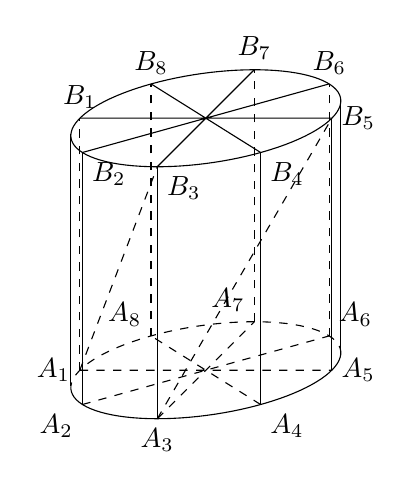
\begin{tikzpicture}[>=latex,scale = 1.6]
\draw [domain = 0:360, samples = 100] plot ({cos(\x)},2,{sin(\x)}); 
\draw ({cos(-atan(sqrt(2)/4))},0,{sin((-atan(sqrt(2)/4)))})  coordinate (R);
\draw [domain = {-atan(sqrt(2)/4)}:{-atan(sqrt(2)/4)+180}, samples = 50] plot ({cos(\x)},0,{sin(\x)}) coordinate (L);
\draw [domain = {-atan(sqrt(2)/4)}:{-atan(sqrt(2)/4)-180}, dashed, samples = 50] plot ({cos(\x)},0,{sin(\x)});
\draw (L) --++ (0,2) (R) --++ (0,2);
\draw ({cos(180)},0,{sin(180)}) node [left] {$A_1$} coordinate (A1);
\draw ({cos(135)},0,{sin(135)}) node [below left] {$A_2$} coordinate (A2);
\draw ({cos(90)},0,{sin(90)}) node [below] {$A_3$} coordinate (A3);
\draw ({cos(45)},0,{sin(45)}) node [below right] {$A_4$} coordinate (A4);
\draw ({cos(0)},0,{sin(0)}) node [right] {$A_5$} coordinate (A5);
\draw ({cos(-45)},0,{sin(-45)}) node [above right] {$A_6$} coordinate (A6);
\draw ({cos(-90)},0,{sin(-90)}) node [above left] {$A_7$} coordinate (A7);
\draw ({cos(-135)},0,{sin(-135)}) node [above left] {$A_8$} coordinate (A8);
\draw [dashed] (A1) --++ (0,2) node [above] {$B_1$} coordinate (B1);
\draw (A2) --++ (0,2) node [below right] {$B_2$} coordinate (B2);
\draw (A3) --++ (0,2) node [below right] {$B_3$} coordinate (B3);
\draw (A4) --++ (0,2) node [below right] {$B_4$} coordinate (B4);
\draw (A5) --++ (0,2) node [right] {$B_5$} coordinate (B5);
\draw [dashed] (A6) --++ (0,2) node [above] {$B_6$} coordinate (B6);
\draw [dashed] (A7) --++ (0,2) node [above] {$B_7$} coordinate (B7);
\draw [dashed] (A8) --++ (0,2) node [above] {$B_8$} coordinate (B8);
\draw (B1) -- (B5) (B2) -- (B6) (B3) -- (B7) (B4) -- (B8);
\draw [dashed] (A1) -- (A5) (A2) -- (A6) (A3) -- (A7) (A4) -- (A8);
\draw [dashed] (A1) -- (B3) (A3) -- (B5);
\end{tikzpicture}
\end{center}
(1) 当圆柱底面半径$r$取何值时, $S$取得最大值? 并求出该最大值(结果精确到$0.01$平方米);\\
(2) 在灯笼内, 以矩形骨架的顶点为点, 安装一些霓虹灯, 当灯笼的底面半径为$0.3$米时, 求图中两根直线$A_1B_3$与$A_3B_5$所在异面直线所成角的大小(结果用反三角函数表示).
\item 若实数$x$、$y$、$m$满足$|x-m|>|y-m|$, 则称$x$比$y$远离$m$.\\
(1) 若$x^2-1$比$1$远离$0$, 求$x$的取值范围;\\
(2) 对任意两个不相等的正数$a$、$b$, 证明: $a^3+b^3$比$a^2b+ab^2$远离$2ab\sqrt {ab}$;\\
(3) 已知函数$f(x)$的定义域$D=\{x| x\ne \dfrac{k\pi }2+\dfrac{\pi }4, \ k\in \mathbf{Z}, \ x\in \mathbf{R}\}$.任取$x\in D$, $f(x)$等于$\sin x$和$\cos x$中远离$0$的那个值.写出函数$f(x)$的解析式, 并指出它的基本性质(结论不要求证明).
\item 已知椭圆$\Gamma$的方程为$\dfrac{x^2}{a^2}+\dfrac{y^2}{b^2}=1$($a>b>0$), 点$P$的坐标为$(-a, b)$.\\
(1) 若直角坐标平面上的点$M$、$A(0, -b)$、$B(a, 0)$满足$\overrightarrow{PM}=\dfrac{1}{2}(\overrightarrow{PA}+\overrightarrow{PB})$, 求点$M$的坐标;\\
(2) 设直线$l_1:y=k_1x+p$交椭圆$\Gamma$于$C$、$D$两点, 交直线$l_2:y=k_2x$于点$E$. 若$k_1\cdot k_2=-\dfrac{b^2}{a^2}$, 证明: $E$为$CD$的中点;\\
(3) 对于椭圆$\Gamma$上的点$Q(a \cos\theta , b \sin\theta )$($0<\theta <\pi$), 如果椭圆$\Gamma$上存在不同的两点$P_1$、$P_2$满足$\overrightarrow{PP_1}+\overrightarrow{PP_2}=\overrightarrow{PQ}$, 写出求作点$P_1$、$P_2$的步骤, 并求出使$P_1$、$P_2$存在的$\theta$的取值范围.
%gk11/23
\item 函数$f(x)=\dfrac 1{x-2}$的反函数为$f^{-1}(x)=$\blank{50}.
\item 若全集$U=\mathbf{R}$, 集合$A=\{x|x\ge 1\}\cup \{x|x\le 0\}$, 则$C_UA=$\blank{50}.
\item 设$m$为常数, 若点$F(0,5)$是双曲线$\dfrac{y^2}m-\dfrac{x^2}9=1$的一个焦点, 则$m=$\blank{50}.
\item 不等式$\dfrac{x+1}x<3$的解为\blank{50}.
\item 在极坐标系中, 直线$\rho (2\cos \theta +\sin \theta)=2$与直线$\rho \cos \theta =1$的夹角大小为\blank{50}.
\item 在相距$2$千米的$A$、$B$两点处测量目标$C$, 若$\angle CAB=75^\circ$, $\angle CBA=60^\circ$, 则$A$、$C$两点之间的距离是\blank{50}千米.
\item 若圆锥的侧面积为$2\pi$, 底面积为$\pi$, 则该圆锥的体积为\blank{50}.
\item 函数$y=\sin (\dfrac{\pi}2+x)\cos (\dfrac{\pi}6-x)$的最大值为\blank{50}.
\item 马老师从课本上抄录一个随机变量$\xi$的概率分布律如下表请小牛同学计算$\xi$的数学期望, 尽管``!''处无法完全看清, 且两个``?''处字迹模糊, 但能肯定这两个``?''处的数值相同. 据此, 小牛给出了正确答案$E\xi=$\blank{50}.
\begin{center}
\begin{tabular}{|c|c|c|c|}
\hline
$x$ & $1$ & $2$ & $3$ \\ \hline
$P(\xi=x)$ & ? & ! & ? \\ \hline
\end{tabular}
\end{center}
\item 行列式$\begin{vmatrix}
a & b  \\ c & d  \end{vmatrix}$($a,b,c,d\in \{-1,1,2\}$)的所有可能值中, 最大的是\blank{50}.
\item 在正三角形$ABC$中, $D$是$BC$上的点, $AB=3$, $BD=1$, 则$\overrightarrow{AB}\cdot \overrightarrow{AD}=$\blank{50}.
\item 随机抽取$9$个同学中, 至少有$2$个同学在同一月出生的概率是\blank{50}(默认每月天数相同, 结果精确到$0.001$).
\item 设$g(x)$是定义在$R$上、以$1$为周期的函数, 若$f(x)=x+g(x)$在$[3,4]$上的值域为$[-2,5]$, 则$f(x)$在区间$[-10,10]$上的值域为\blank{50}.
\item 已知点$O(0,0)$、$Q_0(0,1)$和$R_0(3,1)$, 记$Q_0R_0$的中点为$P_1$, 取$Q_0P_1$和$P_1R_0$中的一条, 记其端点为$Q_1$、$R_1$, 使之满足$(|OQ_1|-2)(|OR_1|-2)<0$; 记$Q_1R_1$的中点为$P_2$, 取$Q_1P_2$和$P_2R_1$中的一条, 记其端点为$Q_2$、$R_2$, 使之满足$(|OQ_2|-2)(|OR_2|-2)<0$; 依次下去, 得到点$P_1,P_2,\cdots ,P_n,\cdots$, 则$\displaystyle\lim_{n\to\infty}|Q_0P_n|=$\blank{50}.
\item 若$a,b\in \mathbf{R}$, 且$ab>0$, 则下列不等式中, 恒成立的是\bracket{20}.
\fourch{$a^2+b^2>2ab$}{$a+b\ge 2\sqrt {ab}$}{$\dfrac 1a+\dfrac 1b>\dfrac 2{\sqrt {ab}}$}{$\dfrac ba+\dfrac ab\ge 2$}
\item 下列函数中, 既是偶函数, 又是在区间$(0,+\infty)$上单调递减的函数为\bracket{20}.
\fourch{$y=\ln \dfrac 1{|x|}$}{$y=x^3$}{$y=2^{|x|}$}{$y=\cos x$}
\item 设$A_1,A_2,A_3,A_4,A_5$是空间中给定的$5$个不同的点, 则使$\overrightarrow{MA_1}+\overrightarrow{MA_2}+\overrightarrow{MA_3}+\overrightarrow{MA_4}+\overrightarrow{MA_5}=\overrightarrow 0$成立的点$M$的个数为\bracket{20}.
\fourch{$0$}{$1$}{$5$}{$10$}
\item 设$\{a_n\}$是各项为正数的无穷数列, $A_i$是边长为$a_i,a_{i+1}$的矩形面积($i=1,2,\cdots$), 则$\{A_n\}$为等比数列的充要条件为\bracket{20}.
\onech{$\{a_n\}$是等比数列}{$a_1,a_3,\cdots ,a_{2n-1},\cdots$或$a_2,a_4,\cdots ,a_{2n},\cdots$是等比数列}{$a_1,a_3,\cdots ,a_{2n-1},\cdots$和$a_2,a_4,\cdots ,a_{2n},\cdots$均是等比数列}{$a_1,a_3,\cdots ,a_{2n-1},\cdots$和$a_2,a_4,\cdots ,a_{2n},\cdots$均是等比数列, 且公比相同}
\item 已知复数$z_1$满足$(z_1-2)(1+\mathrm{i})=1-\mathrm{i}$($\mathrm{i}$为虚数单位), 复数$z_2$的虚部为$2$, $z_1\cdot z_2$是实数, 求$z_2$.
\item 已知函数$f(x)=a\cdot 2^x+b\cdot 3^x$, 其中常数$a,b$满足$ab\ne 0$.
(1) 若$ab>0$, 判断函数$f(x)$的单调性;\\
(2) 若$ab<0$, 求$f(x+1)>f(x)$时$x$的取值范围.
\item 已知$ABCD-A_1B_1C_1D_1$是底面边长为$1$的正四棱柱, $O_1$是$A_1C_1$和$B_1D_1$的交点.
\begin{center}
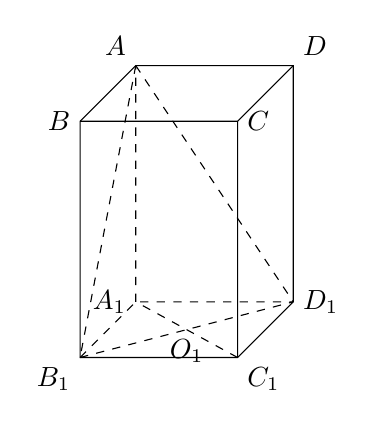
\begin{tikzpicture}[>=latex]
\draw (0,0) node [below left] {$B_1$} coordinate (A) --++ (2,0) node [below right] {$C_1$} coordinate (B) --++ (45:{2/2}) node [right] {$D_1$} coordinate (C)
--++ (0,3) node [above right] {$D$} coordinate (C1)
--++ (-2,0) node [above left] {$A$} coordinate (D1) --++ (225:{2/2}) node [left] {$B$} coordinate (A1) -- cycle;
\draw (A) ++ (2,3) node [right] {$C$} coordinate (B1) -- (B) (B1) --++ (45:{2/2}) (B1) --++ (-2,0);
\draw [dashed] (A) --++ (45:{2/2}) node [left] {$A_1$} coordinate (D) --++ (2,0) (D) --++ (0,3);
\draw [dashed] (A) -- (C) (B) -- (D) (D1) -- (A) (D1) -- (C);
\draw ($(A)!0.5!(C)$) node [below] {$O_1$} coordinate (O1);
\end{tikzpicture}
\end{center}
(1) 设$AB_1$与底面$A_1B_1C_1D_1$所成的角的大小为$\alpha$, 二面角$A-B_1D_1-A_1$的大小为$\beta$. 求证: $\tan \beta =\sqrt 2\tan \alpha$;\\
(2) 若点$C$到平面$AB_1D_1$的距离为$\dfrac 43$, 求正四棱柱$ABCD-A_1B_1C_1D_1$的高.
\item 已知数列$\{a_n\}$和$\{b_n\}$的通项公式分别为$a_n=3n+6$, $b_n=2n+7$($n\in \mathbf{N}^*$), 将集合$\{x|x=a_n,\ n\in \mathbf{N}^*\}\cup \{x|x=b_n,\ n\in \mathbf{N}^*\}$中的元素从小到大依次排列, 构成数列$c_1,c_2,c_3,\cdots ,c_n,\cdots$.\\
(1) 求$c_1,c_2,c_3,c_4$;\\
(2) 求证: 在数列$\{c_n\}$中、但不在数列$\{b_n\}$中的项恰为$a_2,a_4,\cdots ,a_{2n},\cdots$;\\
(3) 求数列$\{c_n\}$的通项公式.
\item 已知平面上的线段$l$及点$P$, 在$l$上任取一点$Q$, 线段$PQ$长度的最小值称为点$P$到线段$l$的距离, 记作$d(P,l)$.\\
(1) 求点$P(1,1)$到线段$l:x-y-3=0$($3\le x\le 5$)的距离$d(P,l)$;\\
(2) 设$l$是长为$2$的线段, 求点集$D=\{P|d(P,l)\le 1\}$所表示图形的面积;\\
(3) 写出到两条线段$l_1,l_2$距离相等的点的集合$\Omega =\{P|d(P,l_1)=d(P,l_2)\}$, 其中$l_1=AB$, $l_2=CD$, $A,B,C,D$是下列三组点中的一组. 对于下列三组点只需选做一种, 满分分别是\textcircled{1} 2分, \textcircled{2} 6分, \textcircled{3} 8分; 若选择了多于一种的情形, 则按照序号较小的解答计分.\\
\textcircled{1}  $A(1,3)$, $B(1,0)$, $C(-1,3)$, $D(-1,0)$;\\
\textcircled{2}  $A(1,3)$, $B(1,0)$, $C(-1,3)$, $D(-1,-2)$;\\
\textcircled{3}  $A(0,1)$, $B(0,0)$, $C(0,0)$, $D(2,0)$.

%gk12/23
\item 计算: $\dfrac{3-\mathrm{i}}{1+\mathrm{i}}=$\blank{50}($\mathrm{i}$为虚数单位).
\item 若集合$A=\{x|2x+1>0\}$, $B=\{x||x-1|<2\}$, 则$A\cap B=$\blank{50}.
\item 函数$f(x)=\begin{vmatrix} 2 & \cos x \\ \sin x & -1\end{vmatrix}$的值域是\blank{50}.
\item 若$\overrightarrow{n}=(-2,1)$是直线$l$的一个法向量, 则$l$的倾斜角的大小为\blank{50}(结果用反三角函数值表示).
\item 在$(x-\dfrac 2x)^6$的二项展开式中, 常数项等于\blank{50}.
\item 有一列正方体, 棱长组成以$1$为首项、$\dfrac 12$为公比的等比数列, 体积分别记为$V_1,V_2,\cdots,V_n,\cdots$, 则$\displaystyle\lim_{n\to\infty}(V_1+V_2+\cdots+V_n)=$\blank{50}.
\item 已知函数$f(x)=\mathrm{e}^{|x-a|}$($a$为常数). 若$f(x)$在区间$[1,+\infty)$上是增函数, 则$a$的取值范围是\blank{50}.
\item 若一个圆锥的侧面展开图是面积为$2\pi$的半圆面, 则该圆锥的体积为\blank{50}.
\item 已知$f(x)+x^2$是奇函数, 且$f(1)=1$, 若$g(x)=f(x)+2$, 则$g(-1)=$\blank{50}.
\item 如图, 在极坐标系中, 过点$M(2,0)$的直线$l$与极轴的夹角$\alpha=\dfrac \pi 6$, 若将$l$的极坐标方程写成$\rho = f(\theta)$的形式, 则$f(\theta)=$\blank{50}.
\begin{center}
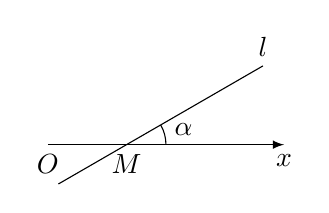
\begin{tikzpicture}[>=latex]
\draw [->] (0,0) node [below] {$O$} -- (3,0) node [below] {$x$} coordinate (x);
\draw (1,0) ++ (-150:1) --++ (30:3) node [above] {$l$} coordinate (l);
\draw (1,0) node [below] {$M$} coordinate (M);
\draw (M) pic [draw, "$\alpha$", angle eccentricity = 1.5] {angle = x--M--l};
\end{tikzpicture}
\end{center}
\item 三位同学参加跳高、跳远、铅球项目的比赛, 若每人都选择其中两个项目, 则有且仅有两人选择的项目完全相同的概率是\blank{50}(结果用最简分数表示).
\item 在平行四边形$ABCD$中, $\angle A=\dfrac \pi 3$, 边$AB$、$AD$的长分别为$2$、$1$, 若$M$、$N$分别是边$BC$、$CD$上的点, 且满足$\dfrac{|\overrightarrow{BM}|}{|\overrightarrow{BC}|}=\dfrac{|\overrightarrow{CN}|}{|\overrightarrow{CD}|}$, 则$\overrightarrow{AM}\cdot \overrightarrow{AN}$的取值范围是\blank{50}.
\item 已知函数$y=f(x)$的图像是折线段$ABC$, 其中$A(0,0)$、$B(\dfrac 12,5)$、$C(1,0)$, 函数$y=xf(x)$($0\le x\le 1$)的图像与$x$轴围成的图形的面积为\blank{50}.
\item 如图, $AD$与$BC$是四面体$ABCD$中互相垂直的棱, $BC=2$, 若$AD=2c$,
且$AB+BD=AC=CD=2a$, 其中$a$、$c$为常数, 则四面体$ABCD$的体积的最大值是\blank{50}.
\begin{center}
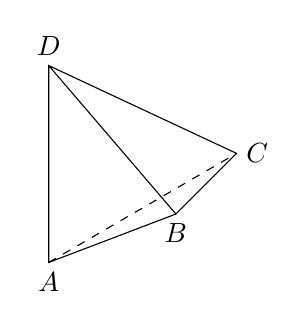
\begin{tikzpicture}[>=latex]
\draw (0,-1,0) node [below] {$A$} coordinate (A);
\draw (0,1.5,0) node [above] {$D$} coordinate (D);
\draw (2,0,1) node [below] {$B$} coordinate (B);
\draw (2,0,-1) node [right] {$C$} coordinate (C);
\draw (A) -- (D) -- (C) -- (B) -- cycle (B) -- (D);
\draw [dashed] (A) -- (C);
\end{tikzpicture}
\end{center}
\item 若$1+2\mathrm{i}$是关于$x$的实系数方程$x^2+bx+c=0$的一个复数根, 则\bracket{20}.
\fourch{$b=2$, $c=3$}{$b=-2$, $c=3$}{$b=-2$, $c=-1$}{$b=2$, $c=-1$}
\item 在$\triangle ABC$中, 若$\sin^2 A+\sin^2 B<\sin^2 C$, 则$\triangle ABC$的形状是\bracket{20}.
\fourch{锐角三角形}{直角三角形}{钝角三角形}{不能确定}
\item 设$10\le x_1<x_2<x_3<x_4\le 10^4$, $x_5=10^5$, 随机变量$\xi_1$取值$x_1,x_2,x_3,x_4,x_5$的概率均为$0.2$, 随机变量$\xi_2$取值$\dfrac{x_1+x_2}2, \dfrac{x_2+x_3}2, \dfrac{x_3+x_4}2, \dfrac{x_4+x_5}2, \dfrac{x_5+x_1}2$的概率也均为$0.2$, 若记$D\xi_1,D\xi_2$分别为$\xi_1,\xi_2$的方差, 则\bracket{20}.
\onech{$D\xi_1>D\xi_2$}{$D\xi_1=D\xi_2$}{$D\xi_1<D\xi_2$}{$D\xi_1$与$D\xi_2$的大小关系与$x_1,x_2,x_3,x_4$的取值有关}
\item 设$a_n=\dfrac 1n\sin \dfrac{n\pi}{25}$, $S_n=a_1+a_2+\cdots+a_n$, 在$S_1,S_2,\cdots,S_{100}$中, 正数的个数是\bracket{20}.
\fourch{$25$}{$50$}{$75$}{$100$}
\item 如图, 在四棱锥$P-ABCD$中, 底面$ABCD$是矩形, $PA\perp$底面$ABCD$, $E$是$PC$的中点.已知$AB=2$, $AD=2$, $PA=2$. 求:
\begin{center}
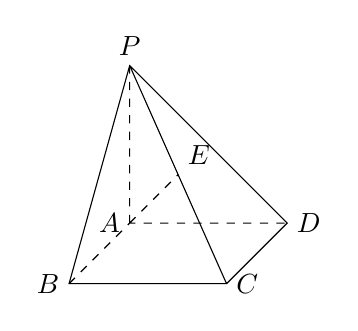
\begin{tikzpicture}[>=latex]
\draw (0,0,0) node [left] {$A$} coordinate (A);
\draw (2,0,0) node [right] {$D$} coordinate (D);
\draw (2,0,2) node [right] {$C$} coordinate (C);
\draw (0,0,2) node [left] {$B$} coordinate (B);
\draw (0,2,0) node [above] {$P$} coordinate (P);
\draw (P) -- (B) -- (C) -- (D) -- cycle (P) -- (C);
\draw [dashed] (A) -- (P) (B) -- (A) -- (D) (A) -- ($(P)!0.5!(C)$) node [above right] {$E$} coordinate (E);
\end{tikzpicture}
\end{center}
(1) 三角形$PCD$的面积;\\
(2) 异面直线$BC$与$AE$所成的角的大小.
\item 已知函数$f(x)=\lg (x+1)$.\\
(1) 若$0<f(1-2x)-f(x)<1$, 求$x$的取值范围;\\
(2) 若$g(x)$是以$2$为周期的偶函数, 且当$0\le x\le 1$时, 有$g(x)=f(x)$, 求函数$y=g(x)$($x\in [1,2]$)的反函数.
\item 海事救援船对一艘失事船进行定位: 以失事船的当前位置为原点, 以正北方向为$y$轴正方向建立平面直角坐标系(以$1$海里为单位长度), 则救援船恰在失事船的正南方向$12$海里$A$处, 如图. 现假设: \textcircled{1} 失事船的移动路径可视为抛物线$y=\dfrac{12}{49}x^2$; \textcircled{2} 定位后救援船即刻沿直线匀速前往救援; \textcircled{3} 救援船出发$t$小时后, 失事船所在位置的横坐标为$7t$.
\begin{center}
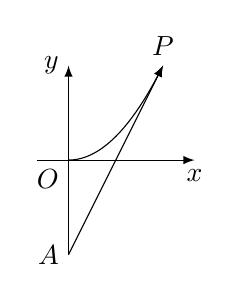
\begin{tikzpicture}[>=latex, scale = 0.4]
\draw [->] (-1,0) -- (4,0) node [below] {$x$};
\draw [->] (0,-3) -- (0,3) node [left] {$y$};
\draw (0,0) node [below left] {$O$};
\draw [domain = 0:3, ->] plot (\x,{pow(\x,2)/3}) node [above] {$P$} coordinate (P);
\draw (0,-3) node [left] {$A$} coordinate (A);
\draw [->] (A) -- (P);
\end{tikzpicture}
\end{center}
(1) 当$t=0.5$时, 写出失事船所在位置$P$的纵坐标. 若此时两船恰好会合, 求救援船速度的大小和方向;\\
(2) 问救援船的时速至少是多少海里才能追上失事船?
\item 在平面直角坐标系$xOy$中, 已知双曲线$C_1:2x^2-y^2=1$.\\
(1) 过$C_1$的左顶点引$C_1$的一条渐近线的平行线, 求该直线与另一条渐近线及$x$轴围成的三角形的面积;\\
(2) 设斜率为$1$的直线$l$交$C_1$于$P$、$Q$两点, 若$l$与圆$x^2+y^2=1$相切, 求证: $OP\perp OQ$;\\
(3) 设椭圆$C_2:4x^2+y^2=1$. 若$M$、$N$分别是$C_1$、$C_2$上的动点, 且$OM\perp ON$, 求证: $O$到直线$MN$的距离是定值.
\item 对于数集$X=\{-1,x_1,x_2,\cdots,x_n\}$, 其中$0\le x_1<x_2<\cdots<x_n$, $n\ge 2$, 定义向量集$Y=\{\overrightarrow{a}|\overrightarrow{a} = (s,t), \ s\in X, \ t\in X\}$, 若对任意$\overrightarrow{a_1}\in Y$, 存在$\overrightarrow{a_2} \in Y$, 使得$\overrightarrow{a_1}\cdot \overrightarrow{a_2}=0$, 则称$X$具有性质$P$. 例如$\{-1,1,2\}$具有性质$P$.\\
(1) 若$x>2$, 且$\{-1,1,2,x\}$具有性质$P$, 求$x$的值;\\
(2) 若$X$具有性质$P$, 求证: $1\in X$, 且当$x_n>1$时, $x_1=1$;\\
(3) 若$X$具有性质$P$, 且$x_1=1$, $x_2=q$($q$为常数), 求有穷数列$x_1,x_2,\cdots,x_n$的通项公式.
%gk13/23
\item 计算: $\displaystyle\lim_{n\to\infty} \dfrac{n+20}{3n+13}=$\blank{50}.
\item 设$m\in \mathbf{R}$, $m^2+m-2+(m^2-1)\mathrm{i}$是纯虚数, 其中$\mathrm{i}$是虚数单位, 则$m=$\blank{50}.
\item 若$\begin{vmatrix}
x^2 & y^2  \\-1 & 1  \end{vmatrix}=\begin{vmatrix}
x & x  \\y & -y  \end{vmatrix}$, 则$x+y=$\blank{50}.
\item 已知$\triangle ABC$的内角$A$、$B$、$C$所对应边分别为$a$、$b$、$c$, 若$3a^2+2ab+3b^2-3c^2=0$, 则角$C$的大小是\blank{50}(结果用反三角函数值表示).
\item 设常数$a\in \mathbf{R}$, 若$(x^2+\dfrac ax)^5$的二项展开式中$x^7$项的系数为$-10$, 则$a=$\blank{50}.
\item 方程$\dfrac 3{3^x-1}+\dfrac 13=3^{x-1}$的实数解为\blank{50}.
\item 在极坐标系中, 曲线$\rho =\cos \theta +1$与$\rho \cos \theta =1$的公共点到极点的距离为\blank{50}.
\item 盒子中装有编号为$1, 2, 3, 4, 5, 6, 7, 8, 9$的九个球, 从中任意取出两个, 则这两个球的编号之积为偶数的概率是\blank{50}(结果用最简分数表示).
\item 设$AB$是椭圆$\Gamma$的长轴, 点$C$在$\Gamma$上, 且$\angle CBA=\dfrac{\pi}4$, 若$AB=4$, $BC=\sqrt 2$, 则$\Gamma$的两个焦点之间的距离为\blank{50}.
\item 设非零常数$d$是等差数列$x_1,x_2,x_3,\cdots ,x_{19}$的公差, 随机变量$\xi$等可能地取值$x_1,x_2,x_3,\cdots ,x_{19}$, 则方差$D\xi =$\blank{50}.
\item 若$\cos x\cos y+\sin x\sin y=\dfrac 12$, $\sin 2x+\sin 2y=\dfrac 23$, 则$\sin (x+y)=$\blank{50}.
\item 设$a$为实常数, $y=f(x)$是定义在$\mathbf{R}$上的奇函数, 当$x<0$时, $f(x)=9x+\dfrac{a^2}x+7$, 若$f(x)\ge a+1$对一切$x\ge 0$成立, 则$a$的取值范围为\blank{50}.
\item 在$xOy$平面上, 将两个半圆弧$(x-1)^2+y^2=1(x\ge 1)$和$(x-3)^2+y^2=1(x\ge 3)$、两条直线$y=1$和$y=-1$围成的封闭图形记为$D$, 如图中阴影部分. 记$D$绕$y$轴旋转一周而成的几何体为$\Omega$, 过$(0,y)$($|y|\le 1$)作$\Omega$的水平截面, 所得截面面积为$4\pi \sqrt {1-y^2}+8\pi$, 试利用祖暅原理、一个平放的圆柱和一个长方体, 得出$\Omega$的体积值为\blank{50}.
\begin{center}
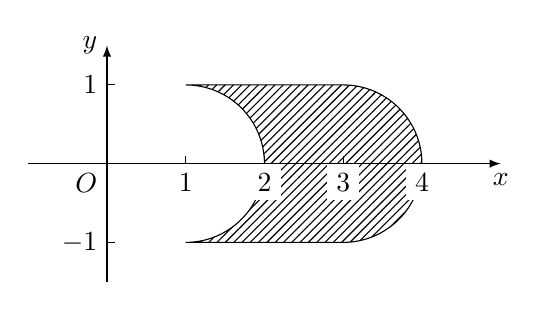
\begin{tikzpicture}[>=latex]
\filldraw [pattern = north east lines] (1,1) -- (3,1) arc (90:-90:1) -- (1,-1) arc (-90:90:1);
\foreach \i in {1,2,3,4}{\draw (\i,0.1) -- (\i,0) node [fill = white, below] {$\i$};};
\draw [->] (-1,0) -- (5,0) node [below] {$x$};
\draw [->] (0,-1.5) -- (0,1.5) node [left] {$y$};
\draw (0,0) node [below left] {$O$};
\foreach \i in  {-1,1}{\draw (0.1,\i) -- (0,\i) node [left] {$\i$};};
\end{tikzpicture}
\end{center}
\item 对区间$I$上有定义的函数$g(x)$, 记$g(I)=\{y|y=g(x),x\in I\}$, 已知定义域为$[0,3]$的函数$y=f(x)$有反函数$y=f^{-1}(x)$, 且$f^{-1}([0,1))=[1,2)$, $f^{-1}((2,4])=[0,1)$, 若方程$f(x)-x=0$有解$x_0$, 则$x_0=$\blank{50}.
\item 设常数$a\in \mathbf{R}$, 集合$A=\{x|(x-1)(x-a)\ge 0\}$, $B=\{x|x\ge a-1\}$, 若$A\cup B=\mathbf{R}$, 则$a$的取值范围为\bracket{20}.
\fourch{$(-\infty ,2)$}{$(-\infty ,2]$}{$(2,+\infty)$}{$[2,+\infty)$}
\item 钱大姐常说``便宜没好货'', 她这句话的意思是: ``不便宜''是``好货''的\bracket{20}.
\twoch{充分条件}{必要条件}{充分必要条件}{既非充分也非必要条件}
\item 在数列$\{a_n\}$中, $a_n=2^n-1$, 若一个$7$行$12$列的矩阵的第$i$行第$j$列的元素$a_{i,j}=a_i\cdot a_j+a_i+a_j$, ($i=1,2,\cdots ,7$; $j=1,2,\cdots ,12$)则该矩阵元素能取到的不同数值的个数为\bracket{20}.
\fourch{$18$}{$28$}{$48$}{$63$}
\item 在边长为$1$的正六边形$ABCDEF$中, 记以$A$为起点, 其余顶点为终点的向量分别为$\overrightarrow{a_1},\overrightarrow{a_2},\overrightarrow{a_3},\overrightarrow{a_4},\overrightarrow{a_5}$; 以$D$为起点, 其余顶点为终点的向量分别为$\overrightarrow{d_1},\overrightarrow{d_2},\overrightarrow{d_3},\overrightarrow{d_4},\overrightarrow{d_5}$. 若$m,M$分别为$(\overrightarrow{a_i}+\overrightarrow{a_j}+\overrightarrow{a_k})\cdot (\overrightarrow{d_r}+\overrightarrow{d_s}+\overrightarrow{d_t})$的最小值、最大值, 其中$\{i,j,k\}\subseteq \{1,2,3,4,5\}$, $\{r,s,t\}\subseteq \{1,2,3,4,5\}$, 则$m,M$满足\bracket{20}.
\fourch{$m=0$, $M>0$}{$m<0$, $M>0$}{$m<0$, $M=0$}{$m<0$, $M<0$}
\item 如图, 在长方体$ABCD-A_1B_1C_1D_1$中, $AB=2$, $AD=1$, $A_1A=1$, 证明直线$BC_1$平行于平面$DA_1C$, 并求直线$BC_1$到平面$D_1AC$的距离.
\begin{center}
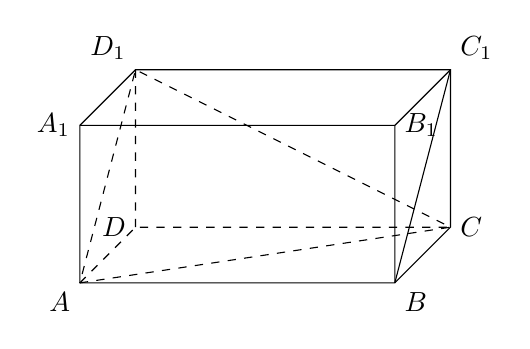
\begin{tikzpicture}[>=latex,scale = 2]
\draw (0,0) node [below left] {$A$} coordinate (A) --++ (2,0) node [below right] {$B$} coordinate (B) --++ (45:{1/2}) node [right] {$C$} coordinate (C)
--++ (0,1) node [above right] {$C_1$} coordinate (C1)
--++ (-2,0) node [above left] {$D_1$} coordinate (D1) --++ (225:{1/2}) node [left] {$A_1$} coordinate (A1) -- cycle;
\draw (A) ++ (2,1) node [right] {$B_1$} coordinate (B1) -- (B) (B1) --++ (45:{1/2}) (B1) --++ (-2,0);
\draw [dashed] (A) --++ (45:{1/2}) node [left] {$D$} coordinate (D) --++ (2,0) (D) --++ (0,1);
\draw (B) -- (C1);
\draw [dashed] (A) -- (C) -- (D1) -- cycle;
\end{tikzpicture}
\end{center}
\item 甲厂以$x$千克/小时的速度运输生产某种产品(生产条件要求$1\le x\le 10$), 每小时可获得利润是$100(5x+1-\dfrac 3x)$元.\\
(1) 要使生产该产品$2$小时获得的利润不低于$3000$元, 求$x$的取值范围;\\
(2) 要使生产$900$千克该产品获得的利润最大, 问: 甲厂应该选取何种生产速度? 并求最大利润.
\item 已知函数$f(x)=2\sin (\omega x)$, 其中常数$\omega >0$.\\
(1) 若$y=f(x)$在$[-\dfrac{\pi }4,\dfrac{2\pi }3]$上单调递增, 求$\omega$的取值范围;\\
(2) 令$\omega =2$, 将函数$y=f(x)$的图像向左平移$\dfrac{\pi }6$个单位, 再向上平移$1$个单位, 得到函数$y=g(x)$的图像, 区间$[a,b]$($a,b\in \mathbf{R}$且$a<b$)满足: $y=g(x)$在$[a,b]$上至少含有$30$个零点, 在所有满足上述条件的$[a,b]$中, 求$b-a$的最小值.
\item 如图, 已知曲线$C_1:\dfrac{x^2}2-y^2=1$, 曲线$C_2:|y|=|x|+1$, $P$是平面上一点, 若存在过点$P$的直线与$C_1,C_2$都有公共点, 则称$P$为``$C_1-C_2$型点''.\\
(1) 在正确证明$C_1$的左焦点是``$C_1-C_2$型点''时, 要使用一条过该焦点的直线, 试写出一条这样的直线的方程(不要求验证);\\
(2) 设直线$y=kx$与$C_2$有公共点, 求证$|k|>1$, 进而证明原点不是``$C_1-C_2$型点'';\\
(3) 求证: 圆$x^2+y^2=\dfrac 12$内的点都不是``$C_1-C_2$型点''.
\item 给定常数$c>0$, 定义函数$f(x)=2|x+c+4|-|x+c|$, 数列$a_1,a_2,a_3,\cdots$满足$a_{n+1}=f(a_n)$, $n\in \mathbf{N}^*$.\\
(1) 若$a_1=-c-2$, 求$a_2$及$a_3$;\\
(2) 求证: 对任意$n\in \mathbf{N}^*$, $a_{n+1}-a_n\ge c$;\\
(3) 是否存在$a_1$, 使得$a_1,a_2,\cdots a_n,\cdots$成等差数列? 若存在, 求出所有这样的$a_1$, 若不存在, 说明理由.

%gk14/23
\item 函数$y=1-2\cos ^2(2x)$的最小正周期是\blank{50}.
\item 若复数$z=1+2\mathrm{i}$, 其中$\mathrm{i}$是虚数单位, 则$(z+\dfrac 1{\overline z})\cdot \overline z=$\blank{50}.
\item 抛物线$y^2=2px$的焦点与椭圆$\dfrac{x^2}{9}+\dfrac{y^2}{5}=1$的右焦点重合, 则该抛物线的准线方程为\blank{50}.
\item 设$f(x)=\begin{cases}x, & x\in (\infty,a),\\ x^2, & x\in [a,+\infty),\end{cases}$若$f(2)=4$, 则$a$的取值范围为\blank{50}.
\item 若实数$x,y$满足$xy=1$, 则$x^2+2y^2$的最小值为\blank{50}.
\item 若圆锥的侧面积是底面积的$3$倍, 则其母线与底面角的大小为\blank{50}(结果用反三角函数值表示).
\item 已知曲线$C$的极坐标方程为$\rho(3\cos\theta-4\sin\theta)=1$, 则$C$与极轴的交点到极点的距离是\blank{50}.
\item 设无穷等比数列$\{a_n\}$的公比为$q$, 若$a_1=\displaystyle\lim_{n\to \infty}(a_3+a_4+\cdots)$, 则$q=$\blank{50}.
\item 若$f(x)=x^\frac 23-x^\frac 12$, 则满足$f(x)<0$的$x$的取值范围是\blank{50}.
\item 为强化安全意识, 某商场拟在未来的连续$10$天中随机选择$3$天进行紧急疏散演练, 则选择的$3$天恰好为连续$3$天的概率是\blank{50}(结果用最简分数表示).
\item 已知互异的复数$a, b$满足$ab\ne 0$, 集合$\{a, b\}=\{a^2,b^2\}$, 则$a+b=$\blank{50}.
\item 设常数$a$使方程$\sin x+\sqrt{3}\cos x=a$在闭区间$[0, 2\pi]$上恰有三个解$x_1,x_2,x_3$, 则$x_1+x_2+x_3=$\blank{50}.
\item 某游戏的得分为$1, 2, 3, 4, 5$, 随机变量$\xi$表示小白玩游戏的得分. 若$E\xi = 4.2$, 则小白得$5$分的概率至少为\blank{50}.
\item 已知曲线$C:x=-\sqrt{4-y^2}$, 直线$l: x=6$. 若对于点$A(m, 0)$, 存在$C$上的点$P$和$l$上的点$Q$使得$\overrightarrow{AP}+\overrightarrow{AQ}=\overrightarrow 0$, 则$m$的取值范围为\blank{50}.
\item 设$a,b\in \mathbf{R}$, 则``$a+b>4$''是``$a>2$且$b>2$''的\bracket{20}.
\twoch{充分条件}{必要条件}{充分必要条件}{既非充分又非必要条件}
\item 如图, 四个棱长为$1$的正方体排成一个正四棱柱, $AB$是一条侧棱, $P_i$($i=1,2,\cdots$)是上底面上其余的八个点, 则$\overrightarrow{AB}\cdot \overrightarrow{AP_i}$($i=1,2,\cdots$)的不同值的个数为\bracket{20}.
\begin{center}
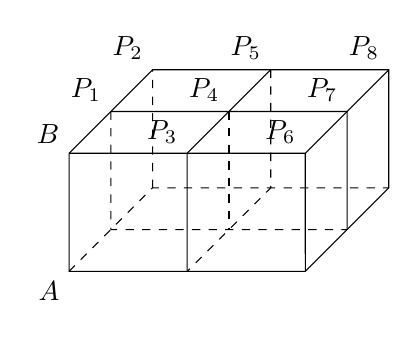
\begin{tikzpicture}[>=latex, scale = 1.5]
\draw (0,0) node [below left] {$A$} coordinate (A) --++ (2,0)  coordinate (B) --++ (45:{2/2})  coordinate (C)
--++ (0,1)  coordinate (C1) node [above left] {$P_8$}
--++ (-2,0)  coordinate (D1) node [above left] {$P_2$} --++ (225:{2/2}) node [above left] {$B$} coordinate (A1) -- cycle;
\draw (A) ++ (2,1)  coordinate (B1) node [above left] {$P_6$} -- (B) (B1) --++ (45:{2/2}) (B1) --++ (-2,0);
\draw [dashed] (A) --++ (45:{2/2})  coordinate (D) --++ (2,0) (D) --++ (0,1);
\draw ($(A1)!0.5!(D1)$) node [above left] {$P_1$} coordinate (P1);
\draw ($(B1)!0.5!(C1)$) node [above left] {$P_7$} coordinate (P7);
\draw ($(A1)!0.5!(B1)$) node [above left] {$P_3$} coordinate (P3);
\draw ($(P1)!0.5!(P7)$) node [above left] {$P_4$} coordinate (P4);
\draw ($(C1)!0.5!(D1)$) node [above left] {$P_5$} coordinate (P5);
\draw (P1) -- (P7) (P3) -- (P5) (P3) --++ (0,-1) coordinate (S) (P7) --++ (0,-1);
\draw [dashed] (P1) --++ (0,-1) --++ (2,0) (P5) --++ (0,-1) -- (S);
\draw [dashed] (P4) --++ (0,-1);
\end{tikzpicture}
\end{center}
\fourch{$1$}{$2$}{$4$}{$8$}
\item 已知$P_1(a_1,b_1)$与$P_2(a_2,b_2)$是直线$y=kx+1$($k$为常数)上两个不同的点, 则关于$x$和$y$的方程组$\begin{cases} a_1x+b_1y=1, \\ a_2x+b_2y=1 \end{cases}$的解的情况是\bracket{20}.
\twoch{无论$k,P_1,P_2$如何, 总是无解}{无论$k,P_1,P_2$如何, 总有唯一解}{存在$k,P_1,P_2$, 使之恰有两解}{存在$k,P_1,P_2$, 使之有无穷多解}
\item 设$f(x)=\begin{cases}(x-a)^2, & x\le 0, \\ x+\dfrac 1x+a, & x>0. \end{cases}$若$f(0)$是$f(x)$的最小值, 则$a$的取值范围为\bracket{20}.
\fourch{$[-1, 2]$}{$[-1, 0]$}{$[1, 2]$}{$[0,2]$}
\item 底面边长为$2$的正三棱锥$P-ABC$, 其表面展开图是三角形$P_1P_2P_3$, 如图, 求$\triangle P_1P_2P_3$的各边长及此三棱锥的体积$V$.
\begin{center}
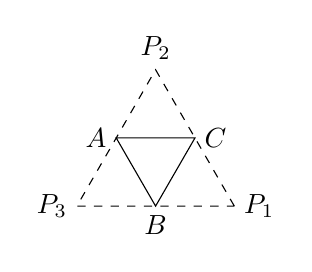
\begin{tikzpicture}[>=latex]
\draw (0,0) node [left] {$A$} coordinate (A);
\draw (1,0) node [right] {$C$} coordinate (C);
\draw (-60:1) node [below] {$B$} coordinate (B);
\draw (A) -- (B) -- (C) -- cycle;
\draw (A) ++ (60:1) node [above] {$P_2$} coordinate (P2);
\draw (A) ++ (-120:1) node [left] {$P_3$} coordinate (P3);
\draw (P3) ++ (2,0) node [right] {$P_1$} coordinate (P1);
\draw [dashed] (P1) -- (P2) -- (P3) -- cycle;
\end{tikzpicture}
\end{center}
\item 设常数$a\ge 0$, 函数$f(x)=\dfrac{2^x+a}{2^x-a}$\\
(1) 若$a=4$, 求函数$y=f(x)$的反函数$y=f^{-1}(x)$;\\
(2) 根据$a$的不同取值, 讨论函数$y=f(x)$的奇偶性, 并说明理由.
\item 如图, 某公司要在$A,B$两地连线上的定点$C$处建造广告牌$CD$, 其中$D$为顶端, $AC$长$35$米, $CB$长$80$米, 设$A,B$在同一水平面上, 从$A$和$B$看$D$的仰角分别为$\alpha$和$\beta$.
(1) 设计中$CD$是铅垂方向, 若要求$\alpha\ge 2\beta$, 问$CD$的长至多为多少(结果精确到$0.01$米)?\\
(2) 施工完成后, $CD$与铅垂方向有偏差, 现在实测得$\alpha=38.12^\circ$, $\beta=18.45^\circ$, 求$CD$的长(结果精确到$0.01$米)?
\begin{center}
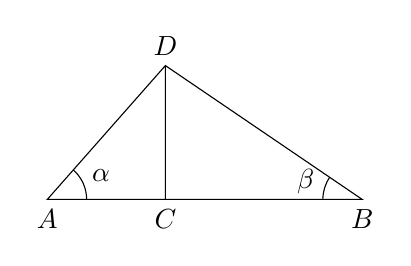
\begin{tikzpicture}[>=latex]
\draw (0,0) node [below] {$A$} coordinate (A);
\draw (4,0) node [below] {$B$} coordinate (B);
\draw (1.5,1.7) node [above] {$D$} coordinate (D);
\draw ($(A)!(D)!(B)$) node [below] {$C$} coordinate (C);
\draw (A) -- (B) -- (D) -- cycle (D) -- (C);
\draw (A) pic ["$\alpha$",draw, angle eccentricity = 1.5] {angle = C--A--D};
\draw (B) pic ["$\beta$",draw, angle eccentricity = 1.5] {angle = D--B--C};
\end{tikzpicture}
\end{center}
\item 在平面直角坐标系$xOy$中, 对于直线$l:ax+by+c=0$和点$P_1(x_1,y_1)$, $P_2(x_2,y_2)$, 记$\eta=(ax_1+by_1+c)(ax_2+by_2+c)$. 若$\eta<0$, 则称点$P_1,P_2$被直线$l$分隔. 若曲线$C$与直线$l$没有公共点, 且曲线$C$上存在点$P_1,P_2$被直线$l$分隔, 则称直线$l$为曲线$C$的一条分隔线.\\
(1) 求证: 点$A(1,2)$, $B(-1,0)$被直线$x+y-1=0$分隔;\\
(2) 若直线$y=kx$是曲线$x^2-4y^2=1$的分隔线, 求实数$k$的取值范围;\\
(3) 动点$M$到点$Q(0,2)$的距离与到$y$轴的距离之积为$1$, 设点$M$的轨迹为$E$, 求证: 通过原点的直线中, 有且仅有一条直线是$E$的分割线.
\item 已知数列$\{a_n\}$满足$\dfrac 13a_n\le a_{n+1}\le 3a_n$, $n\in \mathbf{N}^*$, $a_1=1$.\\
(1) 若$a_2=2$, $a_3=x$, $a_4=9$, 求$x$的取值范围;\\
(2) 若$\{a_n\}$是公比为$q$等比数列. 记$S_n=a_1+a_2+\cdots+a_n$, 若$\dfrac13 S_n\le S_{n+1}\le 3S_n$, $n\in \mathbf{N}^*$, 求$q$的取值范围;\\
(3) 若$a_1,a_2,\cdots,a_k$成等差数列, 且$a_1+a_2+\cdots+a_k=1000$, 求正整数$k$的最大值, 以及$k$取最大值时相应数列$a_1,a_2,\cdots,a_k$的公差.

%gk15/23
\item 设全集$U=\mathbf{R}$. 若集合$A=\{1,2,3,4\}$, $B=\{x|2\le x\le 3\}$, 则$A\cap \overline B=$\blank{50}.
\item 若复数$z$满足$3z+\overline z=1+\mathrm{i}$, 其中$\mathrm{i}$为虚数单位, 则$z=$\blank{50}.
\item 若线性方程组的增广矩阵为$\begin{pmatrix}
2 & 3 & c_1  \\0 & 1 & c_2  \end{pmatrix}$、解为$\begin{cases} x=3, \\ y=5, \end{cases}$, 则$c_1-c_2=$\blank{50}.
\item 若正三棱柱的所有棱长均为$a$, 且其体积为$16\sqrt 3$, 则$a=$\blank{50}.
\item 抛物线$y^2=2px$($p>0$)上的动点$Q$到焦点的距离的最小值为$1$, 则$p=$\blank{50}.
\item 若圆锥的侧面积与过轴的截面面积之比为$2\pi$, 则其母线与轴的夹角的大小为\blank{50}.
\item 方程$\log_2(9^{x-1}-5)=\log_2(3^{x-1}-2)+2$的解为\blank{50}.
\item 在报名的$3$名男教师和$6$名女教师中, 选取$5$人参加义务献血, 要求男、女教师都有, 则不同的选取方式的种数为\blank{50}(结果用数值表示).
\item 已知点$P$和$Q$的横坐标相同, $P$的纵坐标是$Q$的纵坐标的$2$倍, $P$和$Q$的轨迹分别为双曲线$C_1$和$C_2$. 若$C_1$的渐近线方程为$y=\pm \sqrt 3x$, 则$C_2$的渐近线方程为\blank{50}.
\item 设$f^{-1}(x)$为$f(x)=2^{x-2}+\dfrac x2$, $x\in [0,2]$的反函数, 则$y=f(x)+f^{-1}(x)$的最大值为\blank{50}.
\item 在$(1+x+\dfrac 1{x^{2015}})^{10}$的展开式中, $x^2$项的系数为\blank{50}(结果用数值表示).
\item 赌博有陷阱. 某种赌博每局的规则是: 赌客先在标记有$1,2,3,4,5$的卡片中随机摸取一张, 将卡片上的数字作为其赌金(单位: 元); 随后放回该卡片, 再随机摸取两张, 将这两张卡片上数字之差的绝对值的$1.4$倍作为其奖金(单位: 元). 若随机变量$\xi _1$和$\xi _2$分别表示赌客在一局赌博中的赌金和奖金, 则$E \xi _1-E \xi _2=$\blank{50}(元).
\item 已知函数$f(x)=\sin x$. 若存在$x_1$, $x_2$, $\cdots$, $x_m$满足$0\le x_1<x_2<\cdots <x_m\le 6\pi$, 且
$|f(x_1)-f(x_2)|+|f(x_2)-f(x_3)|+\cdots +|f(x_{n-1})-f(x_n)|=12$($m\ge 2$, $m\in \mathbf{N}^*$), 则$m$的最小值为\blank{50}.
\item 在锐角三角形$ABC$中, $\tan A=\dfrac 12$, $D$为边$BC$上的点, $\triangle ABD$与$\triangle ACD$的面积分别为$2$和$4$. 过$D$作$DE \perp AB$于$E$, $DF\perp AC$于$F$, 则$\overrightarrow{DE}\cdot \overrightarrow{DF}=$\blank{50}.
\item 设$z_1$, $z_2\in \mathbf{C}$, 则``$z_1$、$z_2$中至少有一个数是虚数''是``$z_1-z_2$是虚数''的\bracket{20}.
\twoch{充分非必要条件}{必要非充分条件}{充要条件}{既非充分又非必要条件}
\item 已知点$A$的坐标为$(4\sqrt 3,1)$, 将$OA$绕坐标原点$O$逆时针旋转$\dfrac{\pi }3$至$OB$, 则点$B$的纵坐标为\bracket{20}.
\fourch{$\dfrac{3\sqrt 3}2$}{$\dfrac{5\sqrt 3}2$}{$\dfrac{11}2$}{$\dfrac{13}2$}
\item 记方程\textcircled{1}: $x^2+a_1x+1=0$, 方程\textcircled{2}: $x^2+a_2x+2=0$, 方程\textcircled{3}: $x^2+a_3x+4=0$, 其中$a_1,a_2,a_3$是正实数. 当$a_1,a_2,a_3$成等比数列时, 下列选项中, 能推出方程\textcircled{3}无实根的是\bracket{20}.
\twoch{方程\textcircled{1}有实根, 且\textcircled{2}有实根}{方程\textcircled{1}有实根, 且\textcircled{2}无实根}{方程\textcircled{1}无实根, 且\textcircled{2}有实根}{方程\textcircled{1}无实根, 且\textcircled{2}无实根}
\item 设$P_n(x_n,y_n)$是直线$2x-y=\dfrac n{n+1}$($n\in \mathbf{N}^*$)与圆$x^2+y^2=2$在第一象限的交点, 则极限$\displaystyle\lim_{n\to \infty} \dfrac{y_n-1}{x_n-1}=$\bracket{20}.
\fourch{$-1$}{$-\dfrac 12$}{$1$}{$2$}
\item 如图, 在长方体$ABCD-A_1B_1C_1D_1$中, $AA_1=1$, $AB=AD=2$, $E$、$F$分别是$AB$、$BC$的中点. 证明$A_1$、$C_1$、$F$、$E$四点共面, 并求直线$CD_1$与平面$A_1C_1FE$所成的角的大小.
\begin{center}
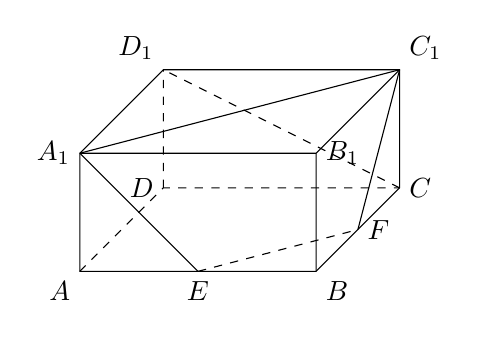
\begin{tikzpicture}[>=latex,scale = 1.5]
\draw (0,0) node [below left] {$A$} coordinate (A) --++ (2,0) node [below right] {$B$} coordinate (B) --++ (45:{2/2}) node [right] {$C$} coordinate (C)
--++ (0,1) node [above right] {$C_1$} coordinate (C1)
--++ (-2,0) node [above left] {$D_1$} coordinate (D1) --++ (225:{2/2}) node [left] {$A_1$} coordinate (A1) -- cycle;
\draw (A) ++ (2,1) node [right] {$B_1$} coordinate (B1) -- (B) (B1) --++ (45:{2/2}) (B1) --++ (-2,0);
\draw [dashed] (A) --++ (45:{2/2}) node [left] {$D$} coordinate (D) --++ (2,0) (D) --++ (0,1);
\draw ($(A)!0.5!(B)$) node [below] {$E$} coordinate (E);
\draw ($(B)!0.5!(C)$) node [right] {$F$} coordinate (F);
\draw [dashed] (E) -- (F) (C) -- (D1);
\draw (A1) -- (E) (C1) -- (F) (A1) -- (C1);
\end{tikzpicture}
\end{center}
\item 如图, $A$, $B$, $C$三地有直道相通, $AB=5$千米, $AC=3$千米, $BC=4$千米. 现甲、乙两警员同时从$A$地出发匀速前往$B$地, 经过$t$小时, 他们之间的距离为$f(t)$(单位: 千米).甲的路线是$AB$, 速度为$5$千米/小时, 乙的路线是$ACB$, 速度为$8$千米/小时. 乙到达$B$地后原地等待. 设$t=t_1$时乙到达$C$地.
\begin{center}
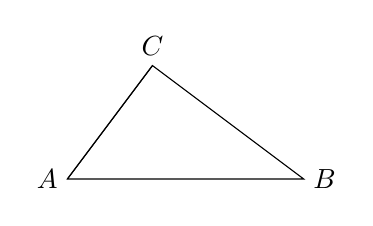
\begin{tikzpicture}[>=latex,scale = 0.6]
\draw (0,0) node [left] {$A$} coordinate (A);
\draw (A) --++ ({atan(4/3)}:3) node [above] {$C$} coordinate (C);
\draw (5,0) node [right] {$B$} coordinate (B);
\draw (A) -- (B) -- (C) -- cycle;
\end{tikzpicture}
\end{center}
(1) 求$t_1$与$f(t_1)$的值;\\
(2) 已知警员的对讲机的有效通话距离是$3$千米.当$t_1\le t\le 1$时, 求$f(t)$的表达式, 并判断$f(t)$在$[t_1,1]$上的最大值是否超过$3$? 说明理由.
\item 已知椭圆$x^2+2y^2=1$, 过原点的两条直线$l_1$和$l_2$分别于椭圆交于$A$、$B$和$C$、$D$, 记得到的平行四边形$ABCD$的面积为$S$.\\
(1) 设$A(x_1,y_1)$, $C(x_2,y_2)$, 用$A$、$C$的坐标表示点$C$到直线$l_1$的距离, 并证明$S=2|x_1y_1-x_2y_1|$;\\
(2) 设$l_1$与$l_2$的斜率之积为$-\dfrac 12$, 求面积$S$的值.
\item 已知数列$\{a_n\}$与$\{b_n\}$满足$a_{n+1}-a_n=2(b_{n+1}-b_n)$, $n\in \mathbf{N}^*$.\\
(1) 若$b_n=3n+5$, 且$a_1=1$, 求数列$\{a_n\}$的通项公式;\\
(2) 设$\{a_n\}$的第$n_0$项是最大项, 即$a_{n_0}>a_n$($n\in \mathbf{N}^*$), 求证: 数列$\{b_n\}$的第$n_0$项是最大项;\\
(3) 设$a_1=\lambda <0$, $b_n=\lambda ^n$($n\in \mathbf{N}^*$), 求$\lambda$的取值范围, 使得$\{a_n\}$有最大值$M$与最小值$m$, 且$\dfrac M m\in (-2,2)$.
\item 对于定义域为$\mathbf{R}$的函数$g(x)$, 若存在正常数$T$, 使得$\cos g(x)$是以$T$为周期的函数, 则称$g(x)$为余弦周期函数, 且称$T$为其余弦周期. 已知$f(x)$是以$T$为余弦周期的余弦周期函数, 其值域为$\mathbf{R}$. 设$f(x)$单调递增, $f(0)=0$, $f(T)=4\pi$.\\
(1) 验证$h(x)=x+\sin \dfrac x3$是以$6\pi$为周期的余弦周期函数;\\
(2) 设$a<b$. 证明对任意$c\in [f(a),f(b)]$, 存在$x_0\in [a,b]$, 使得$f(x_0)=c$;\\
(3) 证明: ``$u_0$为方程$\cos f(x)=1$在$[0,T]$上的解''的充要条件是``$u_0+T$为方程$\cos f(x)=1$在$[T ,2T]$上有解'', 并证明对任意$x\in [0,T]$都有$f(x+T)=f(x)+f(T)$.


%gk16/23
\item 设$x\in \mathbf{R}$, 则不等式$|x-3|<1$的解集为\blank{50}.
\item 设$Z=\dfrac{3+2\mathrm{i}}{\mathrm{i}}$, 其中$\mathrm{i}$为虚数单位, 则$\mathrm{Im}z=$\blank{50}.
\item 已知平行直线$l_1:2x+y-1=0$, $l_2:2x+y+1=0$, 则$l_1,l_2$的距离为\blank{50}.
\item 某次体检, $6$位同学的身高(单位: 米)分别为$1.72$, $1.78$, $1.75$, $1.80$, $1.69$, $1.77$, 则这组数据的中位数是\blank{50}(米).
\item 已知点$(3,9)$在函数$f(x)=1+a^x$的图像上, 则$f(x)$的反函数$f^{-1}(x)=$\blank{50}.
\item 如图, 在正四棱柱$ABCD-A_1B_1C_1D_1$中, 底面$ABCD$的边长为$3$, $BD_1$与底面所成角的大小为$\arctan \dfrac 23$, 则该正四棱柱的高等于\blank{50}.
\begin{center}
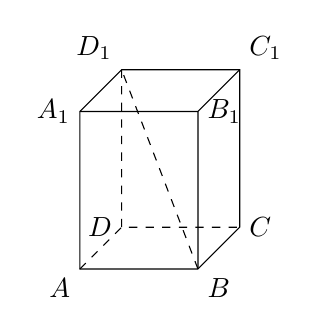
\begin{tikzpicture}[>=latex]
\draw (0,0) node [below left] {$A$} coordinate (A) --++ (1.5,0) node [below right] {$B$} coordinate (B) --++ (45:{1.5/2}) node [right] {$C$} coordinate (C)
--++ (0,2) node [above right] {$C_1$} coordinate (C1)
--++ (-1.5,0) node [above left] {$D_1$} coordinate (D1) --++ (225:{1.5/2}) node [left] {$A_1$} coordinate (A1) -- cycle;
\draw (A) ++ (1.5,2) node [right] {$B_1$} coordinate (B1) -- (B) (B1) --++ (45:{1.5/2}) (B1) --++ (-1.5,0);
\draw [dashed] (A) --++ (45:{1.5/2}) node [left] {$D$} coordinate (D) --++ (1.5,0) (D) --++ (0,2);
\draw [dashed] (B) -- (D1);
\end{tikzpicture}
\end{center}
\item 方程$3\sin x=1+\cos 2x$在区间$[0,2\pi]$上的解为\blank{50}
\item 在$(\sqrt[3]x-\dfrac 2x)^n$的二项式中, 所有项的二项式系数之和为$256$, 则常数项等于\blank{50}.
\item 已知$\triangle ABC$的三边长分别为$3, 5, 7$, 则该三角形的外接圆半径等于\blank{50}.
\item 设$a>0$, $b>0$. 若关于$x,y$的方程组$\begin{cases}
ax+y=1, \\ x+by=1  \end{cases}$无解, 则$a+b$的取值范围是\blank{50}.
\item 无穷数列$\{a_n\}$由$k$个不同的数组成, $S_n$为$\{a_n\}$的前$n$项和.若对任意$n\in \mathbf{N}^*$, $S_n\in \{2,3\}$, 则$k$的最大值为\blank{50}.
\item 在平面直角坐标系中, 已知$A(1, 0)$, $B(0, -1)$, P是曲线$y=\sqrt {1-x^2}$上一个动点, 则$\overrightarrow{BP}\cdot \overrightarrow{BA}$的取值范围是\blank{50}.
\item 设$a,b\in \mathbf{R}$, $c\in [0,2\pi)$, 若对任意实数$x$都有$2\sin (3x-\dfrac{\pi }3)=a\sin (bx+c)$, 则满足条件的有序实数组$(a,b,c)$的组数为\blank{50}.
\item 如图, 在平面直角坐标系$xOy$中, $O$为正八边形$A_1A_2\cdots A_8$的中心, $A_1(1,0)$. 任取不同的两点$A_i,A_j$, 点$P$满足$\overrightarrow{OP}+\overrightarrow{OA_i}+\overrightarrow{OA_j}=\overrightarrow 0$, 则点$P$落在第一象限的概率是\blank{50}.
\begin{center}
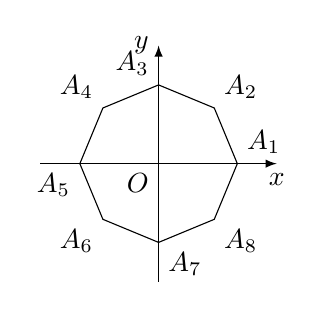
\begin{tikzpicture}[>=latex]
\draw [->] (-1.5,0) -- (1.5,0) node [below] {$x$};
\draw [->] (0,-1.5) -- (0,1.5) node [left] {$y$};
\draw (0,0) node [below left] {$O$};
\draw (0:1) node [above right] {$A_1$} coordinate (A1) -- (45:1) node [above right] {$A_2$} coordinate (A2) -- (90:1) node [above left] {$A_3$} coordinate (A3) -- (135:1) node [above left] {$A_4$} coordinate (A4) -- (180:1) node [below left] {$A_5$} coordinate (A5) -- (225:1) node [below left] {$A_6$} coordinate (A6) -- (270:1) node [below right] {$A_7$} coordinate (A7) -- (315:1) node [below right] {$A_8$} coordinate (A8) -- cycle;
\end{tikzpicture}
\end{center}
\item 设$a\in \mathbf{R}$, 则``$a>1$''是``$a^2>1$''的\bracket{20}.	
\twoch{充分非必要条件}{必要非充分条件}{充要条件}{既非充分也非必要条件}
\item 下列极坐标方程中, 对应的曲线为下图的是\bracket{20}.
\begin{center}
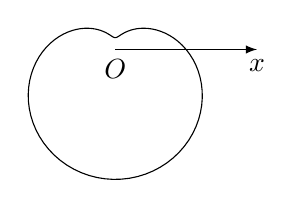
\begin{tikzpicture}[>=latex, scale = 0.15]
\draw [domain = 0:360, samples = 100] plot ({(6-5*sin(\x))*cos(\x)},{(6-5*sin(\x))*sin(\x)});
\draw [->] (0,0) node [below] {$O$} -- (12,0) node [below] {$x$};
\end{tikzpicture}
\end{center}
\fourch{$\rho=6+5\cos\theta$}{$\rho =6+5\sin\theta$}{$\rho =6-5\cos\theta$}{$\rho =6-5\sin \theta$}
\item 已知无穷等比数列$\{a_n\}$的公比为$q$, 前n项和为$S_n$, 且$\displaystyle\lim_{n\to\infty} S_n=S$.下列条件中, 使得$2S_n<S$($n\in \mathbf{N}^*$)恒成立的是\bracket{20}.
\twoch{$a_1>0$, $0.6<q<0.7$}{$a_1<0$, $-0.7<q<-0.6$}{$a_1>0$, $0.7<q<0.8$}{$a_1<0$, $-0.8<q<-0.7$}
\item 设$f(x)$、$g(x)$、$h(x)$是定义域为$\mathbf{R}$的三个函数, 对于命题:\textcircled{1} 若$f(x)+g(x)$、$f(x)+h(x)$、$g(x)+h(x)$均为增函数, 则$f(x)$、$g(x)$、$h(x)$中至少有一个增函数; \textcircled{2} 若$f(x)+g(x)$、$f(x)+h(x)$、$g(x)+h(x)$均是以$T$为周期的函数, 则$f(x)$、$g(x)$、$h(x)$均是以$T$为周期的函数, 下列判断正确的是\bracket{20}.
\twoch{\textcircled{1}和\textcircled{2}均为真命题}{\textcircled{1}和\textcircled{2}均为假命题}{\textcircled{1}为真命题, \textcircled{2}为假命题}{\textcircled{1}为假命题, \textcircled{2}为真命题}
\item 将边长为$1$的正方形$AA_1O_1O$(及其内部)绕的$OO_1$旋转一周形成圆柱, 如图, $\overset\frown{AC}$长为$\dfrac 23\pi$, $\overset\frown{A_1B_1}$长为$\dfrac{\pi }3$, 其中$B_1$与$C$在平面$AA_1O_1O$的同侧.
\begin{center}
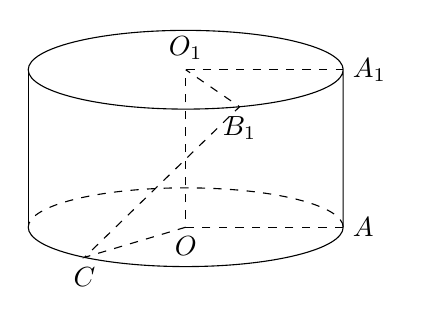
\begin{tikzpicture}[>=latex]
\draw (2,0) node [right] {$A$} coordinate (A) arc (0:-180:2 and 0.5);
\draw [dashed] (2,0) arc (0:180:2 and 0.5);
\draw (A) --++ (0,2) node [right] {$A_1$} coordinate (A1) arc (0:360:2 and 0.5);
\draw (-2,0) -- (-2,2);
\draw (0,0) node [below] {$O$} coordinate (O) (0,2) node [above] {$O_1$} coordinate (O1);
\draw [dashed] (A) -- (O) -- (O1) -- (A1);
\draw ({2*cos(-130)},{0.5*sin(-130)}) node [below] {$C$} coordinate (C);
\draw (0,2) ++ ({2*cos(-70)},{0.5*sin(-70)}) node [below] {$B_1$} coordinate (B1);
\draw [dashed] (O) -- (C) -- (B1) -- (O1);
\end{tikzpicture}
\end{center}
(1) 求三棱锥$C-O_1A_1B_1$的体积;\\
(2) 求异面直线$B_1C$与$AA_1$所成的角的大小.
\item 有一块正方形菜地$EFGH$, $EH$所在直线是一条小河, 收货的蔬菜可送到$F$点或河边运走. 于是, 菜地分为两个区域$S_1$和$S_2$, 其中$S_1$中的蔬菜运到河边较近, $S_2$中的蔬菜运到$F$点较近, 而菜地内$S_1$和$S_2$的分界线$C$上的点到河边与到$F$点的距离相等, 现建立平面直角坐标系, 其中原点$O$为$EF$的中点, 点$F$的坐标为$(1, 0)$, 如图.
\begin{center}
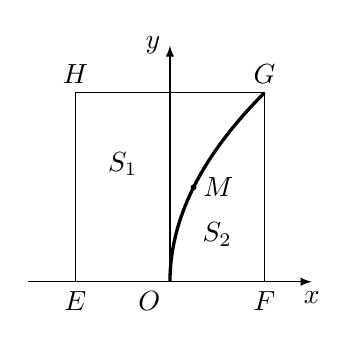
\begin{tikzpicture}[>=latex,scale = 0.6]
\draw [->] (-3,0) -- (3,0) node [below] {$x$};
\draw [->] (0,0) -- (0,5) node [left] {$y$};
\draw (0,0) node [below left] {$O$};
\draw (-2,0) node [below] {$E$} coordinate (E) rectangle (2,4) node [above] {$G$} coordinate (G);
\draw (2,0) node [below] {$F$} coordinate (F);
\draw (-2,4) node [above] {$H$} coordinate (H);
\draw (-1,2.5) node {$S_1$};
\draw (1,1) node {$S_2$};
\draw [very thick, domain = 0:4, samples = 100] plot ({pow(\x,2)/8},\x);
\filldraw ({1/2},2) circle (0.05) node [right] {$M$};
\end{tikzpicture}
\end{center}
(1) 求菜地内的分界线$C$的方程;\\
(2) 菜农从蔬菜运量估计出$S_1$面积是$S_2$面积的两倍, 由此得到$S_1$面积的``经验值''为$\dfrac 83$. 设$M$是$C$上纵坐标为$1$的点, 请计算以$EH$为一边、另一边过点$M$的矩形的面积, 及五边形$EOMGH$的面积, 并判断哪一个更接近于$S_1$面积的经验值.
\item 双曲线$x^2-\dfrac{y^2}{b^2}=1(b>0)$的左、右焦点分别为$F_1$、$F_2$, 直线$l$过$F_2$且与双曲线交于$AB$两点.\\
(1) 若$l$的倾斜角为$\dfrac{\pi }2$, $\triangle F_1AB$是等边三角形, 求双曲线的渐近线方程;\\
(2) 设$b=\sqrt 3$, 若$l$的斜率存在, 且$(\overrightarrow{F_1A}+\overrightarrow{F_1B})\cdot \overrightarrow{AB}=0$, 求$l$的斜率.
\item 已知$a\in \mathbf{R}$, 函数$f(x)=\log_2(\dfrac 1x+a)$.\\
(1) 当$a=5$时, 解不等式$f(x)>0$;\\
(2) 若关于$x$的方程$f(x)-\log_2[(a-4)x+2a-5]=0$的解集中恰好有一个元素, 求$a$的取值范围;\\
(3) 设$a>0$, 若对任意$t\in [\dfrac 12,1]$, 函数$f(x)$在区间$[t,t+1]$上的最大值与最小值的差不超过$1$, 求$a$的取值范围.
\item 若无穷数列$\{a_n\}$满足: 只要$a_p=a_q$($p,q\in \mathbf{N}^*$), 必有$a_{p+1}=a_{q+1}$, 则称$\{a_n\}$具有性质$P$.\\
(1) 若$\{a_n\}$具有性质$P$, 且$a_1=1,a_2=2,a_4=3,a_5=2$, $a_6+a_7+a_8=21$, 求$a_3$;\\
(2) 若无穷数列$\{b_n\}$是等差数列, 无穷数列$\{c_n\}$是公比为正数的等比数列, $b_1=c_5=1$, $b_5=c_1=81$, $a_n=b_n+c_n$. 判断$\{a_n\}$是否具有性质$P$, 并说明理由;\\
(3) 设$\{b_n\}$是无穷数列, 已知$a_{n+1}=b_n+\sin a_n$($n\in \mathbf{N}^*)$. 求证: ``对任意$a_1$, $\{a_n\}$都具有性质$P$''的充要条件为``$\{b_n\}$是常数列''.


\end{enumerate}





\iffalse










\fi

\end{document}